
\subsection*{3.6 Loci}
Loci are the set of points that satisfy a specific condition or rule. They are used to describe the path traced by moving points under given constraints in geometry.

\textbf{Key Concepts:}
\begin{itemize}
	\item \textbf{Definition of a Locus:} A locus is the path traced by a point that moves according to a specific condition or rule.
	\item \textbf{Some Standard Loci:}
	\begin{itemize}
		\item \textbf{Locus of a Point at a Fixed Distance from Another Point:} This is a circle with the fixed point as the center and the given distance as the radius.
		\item \textbf{Locus of Points Equidistant from Two Points:} This is the perpendicular bisector of the line segment joining the two points. Perpendicular bisector to a line PQ is a line passing through midpoint of P and Q and perpendicular to PQ.
		\begin{center}
			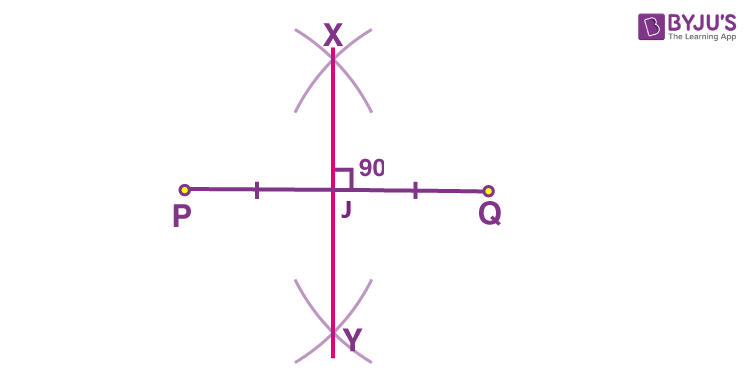
\includegraphics[width=0.6\textwidth]{3.8.png}
		\end{center}
		\item \textbf{Locus of Points Equidistant from Two Intersecting Lines:} This is the angle bisector of the angles formed by the intersecting lines.
		\begin{center}
			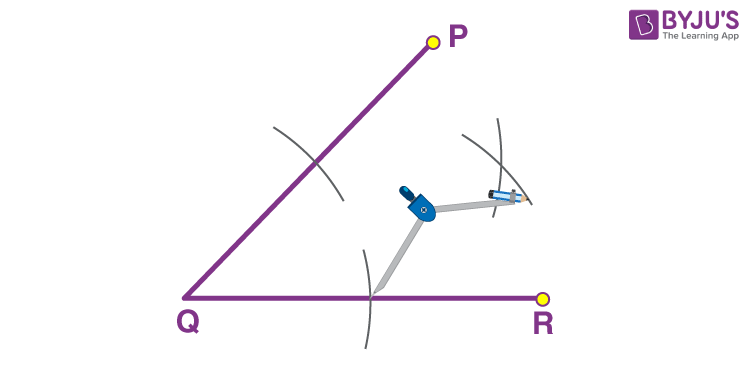
\includegraphics[width=0.6\textwidth]{3.9.png}
		\end{center}
		\item \textbf{Locus of a Point at a Fixed Distance from a Line:} This consists of two parallel lines at the given distance from the original line, one on either side.
	\end{itemize}
	\item \textbf{Real-Life Applications:} Loci are applied in navigation, construction, and design to determine paths or boundaries.
\end{itemize}

\textbf{Examples:}

\begin{flushleft}
	\textbf{Example 1: Describe the locus of points equidistant from two fixed points $A$ and $B$.}
	
	\vspace{0.5cm}
	\textbf{Solution:}
	\vspace{0.5cm}
	
	The locus of points equidistant from $A$ and $B$ is the perpendicular bisector of the line segment joining $A$ and $B$.
\end{flushleft}

\begin{flushleft}
	\textbf{Example 2: Describe the locus of points equidistant from two intersecting lines.}
	
	\vspace{0.5cm}
	\textbf{Solution:}
	\vspace{0.5cm}
	
	The locus of points equidistant from two intersecting lines is the pair of angle bisectors of the angles formed by the lines.
\end{flushleft}

\begin{flushleft}
	\textbf{Example 3: A point $P$ moves such that it is always $5 \, \text{cm}$ away from a fixed point $O$. Describe and sketch the locus of $P$.}
	
	\vspace{0.5cm}
	\textbf{Solution:}
	\vspace{0.5cm}
	
	The locus of $P$ is a circle with center $O$ and radius $5 \, \text{cm}$.
\end{flushleft}

\begin{flushleft}
	\textbf{Example 4: A point $P$ moves such that it is always $3 \, \text{cm}$ away from a straight line $L$. Describe and sketch the locus of $P$.}
	
	\vspace{0.5cm}
	\textbf{Solution:}
	\vspace{0.5cm}
	
	The locus of $P$ consists of two parallel lines, each $3 \, \text{cm}$ away from $L$, one on each side.
\end{flushleft}

\begin{flushleft}
	\textbf{Example 5: A point $P$ moves such that it is equidistant from two fixed points $A$ and $B$ and also equidistant from two intersecting lines $L_1$ and $L_2$. Describe the locus of $P$.}
	
	\vspace{0.5cm}
	\textbf{Solution:}
	\vspace{0.5cm}
	
	The locus of $P$ is the intersection of the perpendicular bisector of the line segment $AB$ and the angle bisectors of the angles formed by the intersecting lines $L_1$ and $L_2$.
\end{flushleft}